\documentclass{beamer}
\usepackage{ragged2e}
\usepackage{graphicx}
\usepackage{xcolor}
\usepackage{algorithm}
\usepackage[noend]{algpseudocode}
% Theme
\usetheme[block=fill, progressbar=frametitle]{metropolis} % Choose a theme (e.g., "Madrid", "Warsaw", "CambridgeUS", "Boadilla", etc.)
\usecolortheme{spruce}

\setbeamercolor{background canvas}{bg=white}
% Title
\title{Rectangular Partitioning of Rectilinear Polygons}
\subtitle{Exercise 15}
\author{Alexandre Ros}
\date{\today}

% Colors
\definecolor{concave}{RGB}{160,32,240} % Define a custom color named "mycolor"
\definecolor{convex}{RGB}{139,0,0} % Define a custom color named "mycolor"
\definecolor{filling}{RGB}{72,116,94} % Define a custom color named "mycolor"

% Begin the document
\begin{document}

% Title page
\frame{\titlepage}

% Table of Contents
% \begin{frame}
%    \frametitle{Table of Contents}
%    \tableofcontents
%\end{frame}

% Section 1
\section{Introduction to the problem}

\begin{frame}{Introduction}
	\begin{block}{Exercise 15}
	\textbf{Decompose a rectilinear polygon into rectangles}, using segments aligned with the edges of the polygon.
The algorithm must produce the \textbf{minimum number of pieces}, and the output must give a
complete description of the partition.
	\end{block}
	\begin{block}{Input}
	A polygon whose sides meet at right angles.
	\end{block}  
	\begin{block}{Output}
	A \textbf{partition} of the polygon into rectangles, with no overlaps.
	\end{block}
	
	We will call this problem $MNC$ (minimal nonoverlapping cover).
\end{frame}

\begin{frame}{Examples}
\begin{figure}
\centering
  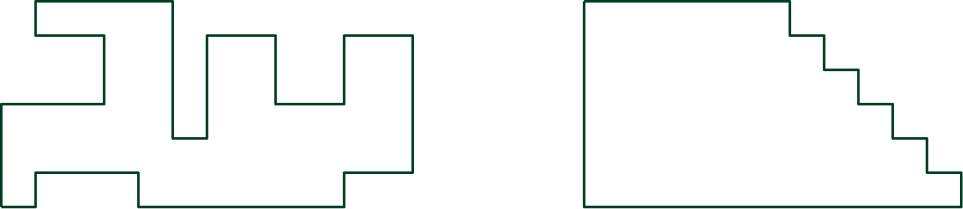
\includegraphics[width=.8\textwidth]{"./rect1.png"}
  \caption{Two rectilinear polygons.}
     \label{fig:question}
\end{figure}
\begin{figure}
\centering
  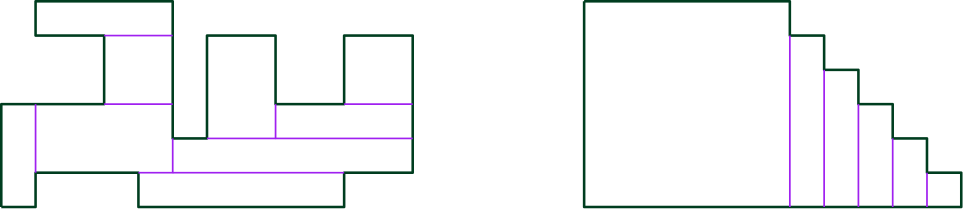
\includegraphics[width=.8\textwidth]{"./rec1sol.png"}
  \caption{A minimum partition of both.}
     \label{fig:question}
\end{figure}

\end{frame}


% Section 2
\section{Preliminaries}

\begin{frame}[t]{Concave and convex vertices}
	In a rectilinear polygon, we can distinguish between concave and convex vertices.
	
    \begin{itemize}
        \item A vertex is said to be \textcolor{concave}{\textbf{concave}} if its interior angle is over 180°.
        \item A vertex is said to be \textcolor{convex}{\textbf{convex}} if its interior angle is under 180°.
    \end{itemize}
    \vspace{10px}
\begin{figure}
\centering
  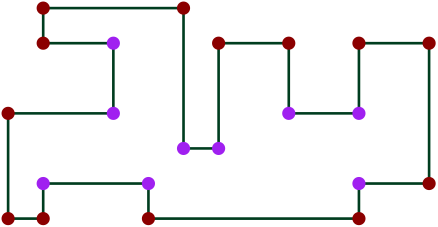
\includegraphics[width=.6\textwidth]{"./concave.png"}
  \caption{Convex (red) and concave (purple) vertices.}
     \label{fig:question}
\end{figure}

\end{frame}

\begin{frame}[t]{Co-vertical, co-horizontal and chords}	
    \begin{itemize}
        \item Two vertices $(x_1, y_1)$, $(x_2, y_2)$ that share no edge are \textbf{co-vertical} $\iff y_1 = y_2$ and \textbf{co-horizontal} $\iff x_1 = x_2$. 
        \item A \textbf{chord} is a segment fully contained inside the polygon that connects two co-horizontal or co-vertical vertices.
    \end{itemize}
    \vspace{10px}
\begin{figure}
\centering
  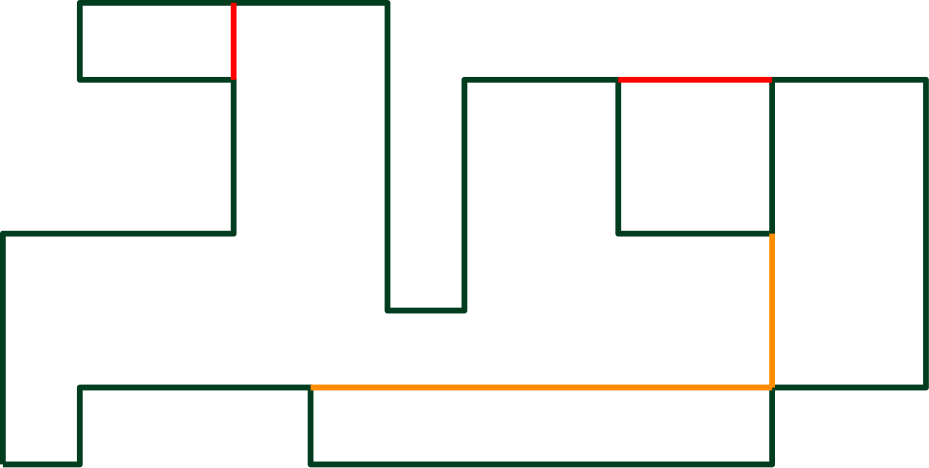
\includegraphics[width=.6\textwidth]{"./chords.png"}
  \caption{Examples of chords (orange) and \textbf{not} chords (red).}
     \label{fig:question}
\end{figure}

\end{frame}


\section{Chord-less polygons}

\begin{frame}[t]{Concave vertices observations}	
	Suppose, for now, that there are no chords in polygon $P$.

	\begin{block}{Observation \#1}
	$P$ is a rectangle $\iff$ $P$ has exactly four convex vertices.
	\end{block}  

	\begin{block}{Observation \#2}
	A concave vertex must be a vertex of two rectangles of the partition. See example below.
	\end{block}  
\begin{figure}

\centering
  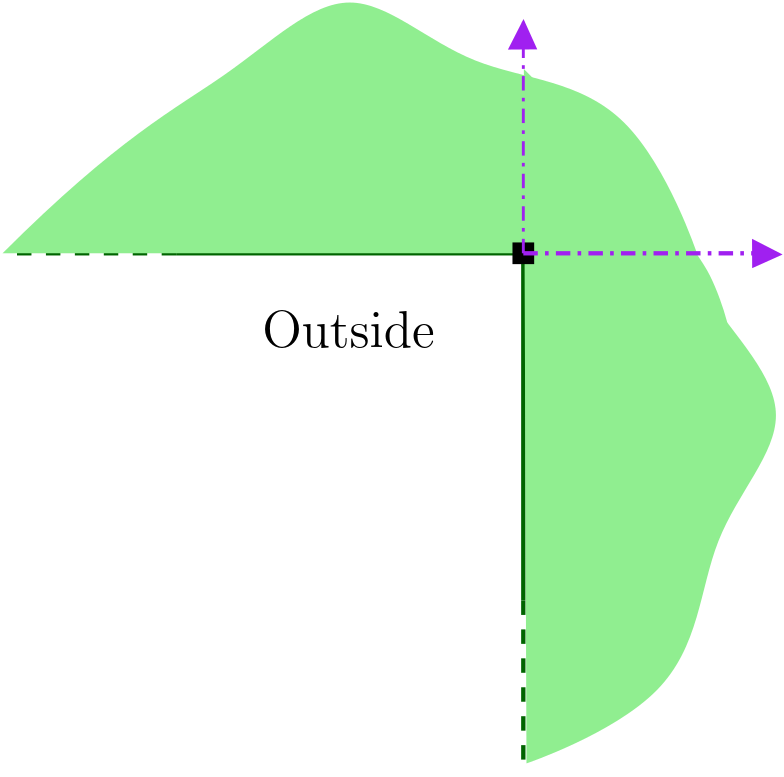
\includegraphics[width=.6\textwidth]{"./direccio.png"}
  \caption{Concave vertex.}
     \label{fig:question}
\end{figure}


\end{frame}

\begin{frame}[t]{Algorithm for chord-less polygons}	
	\begin{block}{Observation \#3}
	If $P$ is not a rectangle then it must have at least one concave vertex.
	\end{block}  

	\begin{block}{Idea to solve the problem}
	For each concave vertex, extend its vertical edge until it hits another edge.
	\textit{If it hits a vertex, then that extension is a chord!}
	\end{block}  
\begin{figure}

\centering
  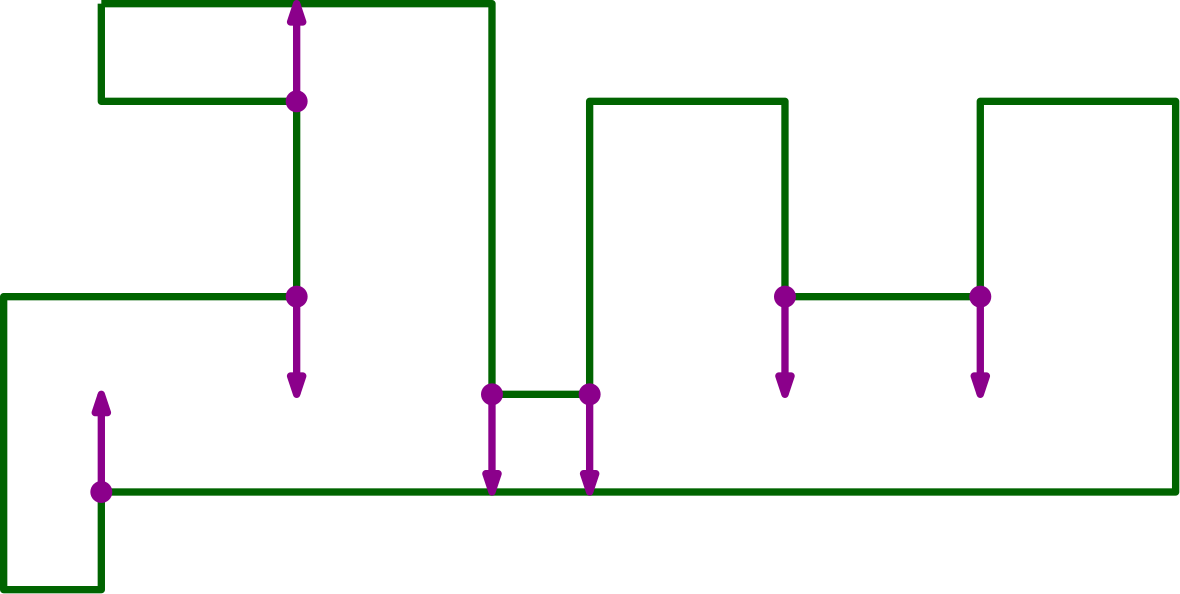
\includegraphics[width=.5\textwidth]{"./launchrays.png"}
  \caption{Chord-less polygons optimal solution.}
     \label{fig:question}
\end{figure}

\end{frame}

\begin{frame}[t]{Algorithm for chord-less polygons}	

  \begin{algorithm}[H] % H option forces the algorithm to stay in place
    \caption{Chord-less MNC in $O(n \log n)$}
    \begin{algorithmic}
      % Your algorithm code goes here
      \Procedure{MNC}{$P$}
      \State $E \leftarrow \emptyset$; $R \leftarrow \emptyset$
        \State $L \leftarrow $ sorted vertices of $P$ by x-coordinate¹.
        \For{each vertex $v$ in $P$}
        \State Insert $v$ to $E$ in position, delete position if duplicate.
        \If{$v$ is concave}
        	  \State Extend vertical edge.
          \State Insert to $R$ the vertical edge.
          \EndIf
        \EndFor
        \State Return $R$ as the paritioning edges of $P$.
      \EndProcedure
    \end{algorithmic}
  \end{algorithm}	
	¹ If using y-coordinate as tiebreaker, we can read pairs of vertices at a time (vertical edges). 

\end{frame}

\foreach \i in {0,1,2,3,4,5,6,7,8}{
  \begin{frame}[t]{Algorithm for chord-less polygons}
    \centering
    \includegraphics[width=\textwidth]{sweep\i.png}
  \end{frame}
}

\section{Polygons with chords}


\begin{frame}[t]{Polygons with chords}	
	\begin{block}{Problem \#1}
	Suppose there are two co-horizontal vertices which form a chord.
	We may prefer joining that chord rather than extending the vertical edge.
	\end{block}  
	
    \centering
    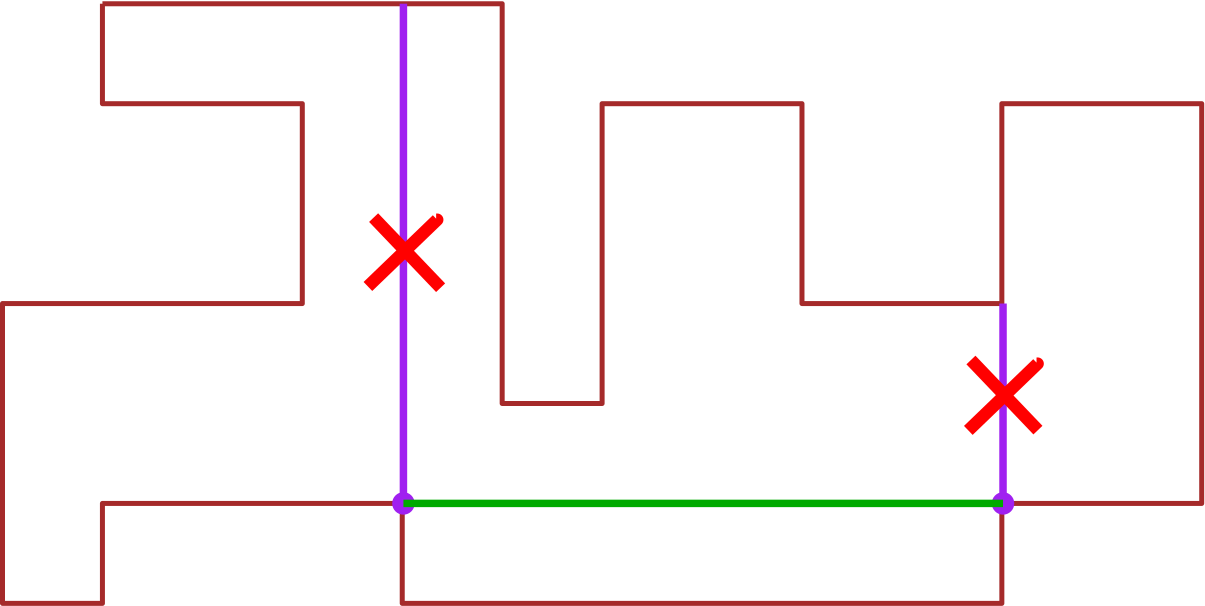
\includegraphics[width=0.7\textwidth]{problem.png}

	We would end up with one more rectangle!

\end{frame}

\begin{frame}[t]{Polygons with chords}	
	\begin{block}{Problem \#2}
	If we drew all chords, there may be intersections.
	\end{block}  
	\vspace{10px}
    \centering
    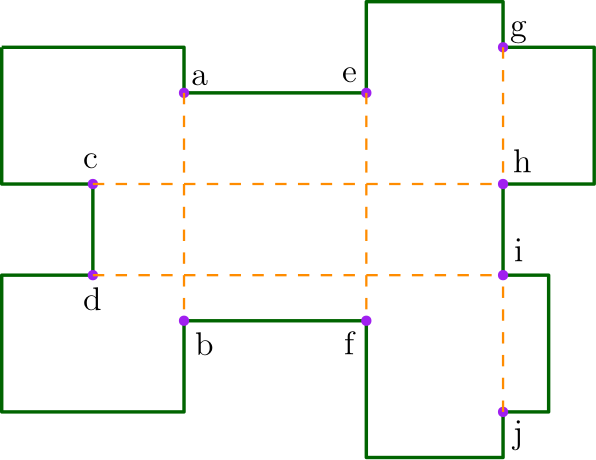
\includegraphics[width=0.6\textwidth]{intersect0.png}

	Chords $ab$ and $ch$ intersect. So do chords $ij$ and $di$.

\end{frame}

\begin{frame}[t]{Polygons with chords}	
	\begin{block}{Solution}
	Draw the largest set of non-intersecting chords. 
	After this step, no chords can remain.
    The remaining sub-polygons can be partitioned as usual.  

	\end{block}  
	\vspace{5px}
    \centering
    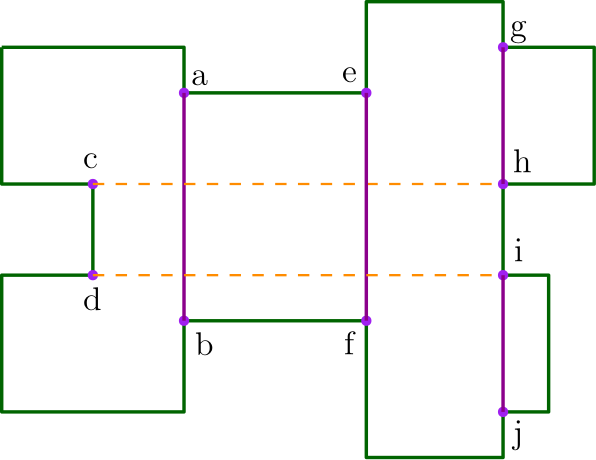
\includegraphics[width=0.6\textwidth]{intersect1.png}

\end{frame}


\begin{frame}[t]{Polygons with chords}	
	\begin{block}{Theorem}
	A rectilinear polygon $R$ has a minimum partition of order $N - L + 1$, where
	
	
	$N = $ Total number of concave vertices on the boundary of $R$.
	$L = $ Maximum number of nonintersecting chords.

	\end{block}  
	\centering
    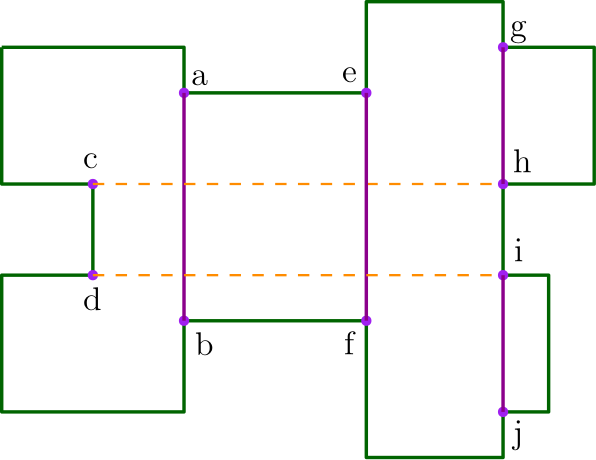
\includegraphics[width=0.43\textwidth]{intersect1.png}
    
    $N = 10$ and $L = 4$ therefore the optimal order is 7.

\end{frame}

\begin{frame}[t]{Finding the largest set of nonintersecting chords}	
	\begin{block}{Process}
	Construct a bipartite graph, with vertices $v_i$ for vertical chords, $h_i$ for horizontal chords, and edges $\{v_i, h_j\}$ if $v_i$ and $h_j$ intersect.
	\end{block}

\end{frame}


% Section 3
\section{Conclusion}

\begin{frame}
    \frametitle{Conclusion}
    \begin{itemize}
        \item Summarize key points.
        \item Highlight takeaways.
    \end{itemize}
\end{frame}

% Additional slides, if needed

% Thank you slide
\begin{frame}
    \frametitle{Thank You}
    \centering
    \Huge Thank you for your attention!
\end{frame}

\end{document}
